\documentclass{article}

% Language setting
% Replace `english' with e.g. `spanish' to change the document language
\usepackage[english]{babel}
\usepackage{float} 
% Set page size and margins
% Replace `letterpaper' with `a4paper' for UK/EU standard size
\usepackage[letterpaper,top=2cm,bottom=2cm,left=3cm,right=3cm,marginparwidth=1.75cm]{geometry}

% Useful packages
\usepackage{amsmath}
\usepackage{graphicx}
\usepackage[colorlinks=true, allcolors=blue]{hyperref}

\title{Emotional Classification of Twitter Comments Enhanced by Data Augmentation}
\author{Chengkun Yang, Xiao Huang, Yue Yu, Yitao Shi, and Teng-yu (Echo) Hsiao}
\date{April 27, 2025}

\begin{document}
\maketitle

\section{Introduction}

This project aims to develop and refine a natural language processing (NLP) model for the classification of emotional content in user comments on X (formerly known as Twitter). Specifically, we seek to categorize tweets into six discrete emotional states: joy, sadness, anger, love, fear, and surprise. As social media platforms have become principal forums for public discourse, the ability to extract emotional cues from user-generated content offers valuable insights into public sentiment trends, user behavior, and psychological well-being at scale.

Text-based emotion classification plays a crucial role across a wide range of applications, including social media monitoring, customer feedback analysis, and mental health assessment. However, building effective emotion classification models remains challenging due to the informal language, abbreviations, and contextual ambiguities prevalent in social media data. Furthermore, the limited availability of labeled emotional datasets often constrains model performance.

To address these challenges, we incorporated data augmentation techniques based on large language models (LLMs) to expand our training dataset, aiming to improve model generalization and enhance classification accuracy. By systematically evaluating models trained with varying amounts of augmented data, we investigated the impact of data augmentation on overall performance. Our findings demonstrate that, through rigorous data cleaning and strategic data augmentation, machine learning approaches can effectively classify emotions even within small-scale datasets. These results highlight the potential for broader applications in real-world emotion-aware systems and contribute to ongoing research efforts in low-resource text classification.

This final report summarizes the full workflow of the project, including data collection, preprocessing, exploratory data analysis, model development, augmentation strategies, evaluation, and key findings.



\section{Dataset Collection}

We collected Twitter user comments using the Twitter API via a developer account. A custom program (developed using the Tweepy library~\cite{tweepy}) was created to crawl tweets associated with six emotional categories: joy, love, fear, anger, surprise, and sad. Specifically, for each category, 250 tweets were extracted by identifying tweets authored with the corresponding tag. If a tweet contained the specified emotional tag in the author's metadata, it was retrieved and assigned to the associated category.

Following collection, a data cleaning process was conducted to improve dataset quality. Incomplete sentences, non-English inputs, and special characters were removed. After cleaning, 100 tweets were randomly sampled from each category to form the original dataset. A final human check was performed to ensure the accuracy and quality of the dataset.

To address the limited size of the original dataset, we applied data augmentation using ChatGPT-4o. For each emotional category, 900 additional synthetic sentences were generated, resulting in an expanded dataset with a more balanced and enriched representation of emotional expressions. This complete dataset served as the foundation for model training and evaluation in subsequent experiments.

\section{Dataset Description}
The dataset comprises tweets collected via the Twitter API and amplified by ChatGPT-4o. Each entry includes tweet text and metadata. We labeled the data with one of several emotion categories: \emph{joy}, \emph{sadness}, \emph{fear}, \emph{anger}, \emph{love}, and \emph{surprise}. Each label contained 100 cleaned original tweets and labels, and 900 synthetic tweets and labels. Key preprocessing steps include:

\begin{itemize}
    \item \textbf{Tokenization}: Splitting tweets into individual tokens.
    \item \textbf{Text Normalization}: Converting all text to lowercase and removing URLs, non-English inputs, special characters, and emojis where appropriate.
    \item \textbf{Handling Class Imbalance and Data Augmentation}: We selected 100 tweets for each label and applied data augmentation using ChatGPT-4o. The prompt we used was: "Generate 100 emotion-labeled sentences under the [category]. Each sentence should be 1–2 sentences long and include clear emotional cues through concrete details and imagery. The tone should be natural and grounded in daily experiences. [Strict] Do not repeat with the previous generated sentences." And we repeated this process 9 times in total for each label.
\end{itemize}

These steps were guided by best practices in NLP to ensure the resultant dataset is clean and representative. We have retained some representative samples in the GitHub repository for illustration.

\section{Model Evaluation and Results}

% \begin{figure}[H]
%     \centering
%     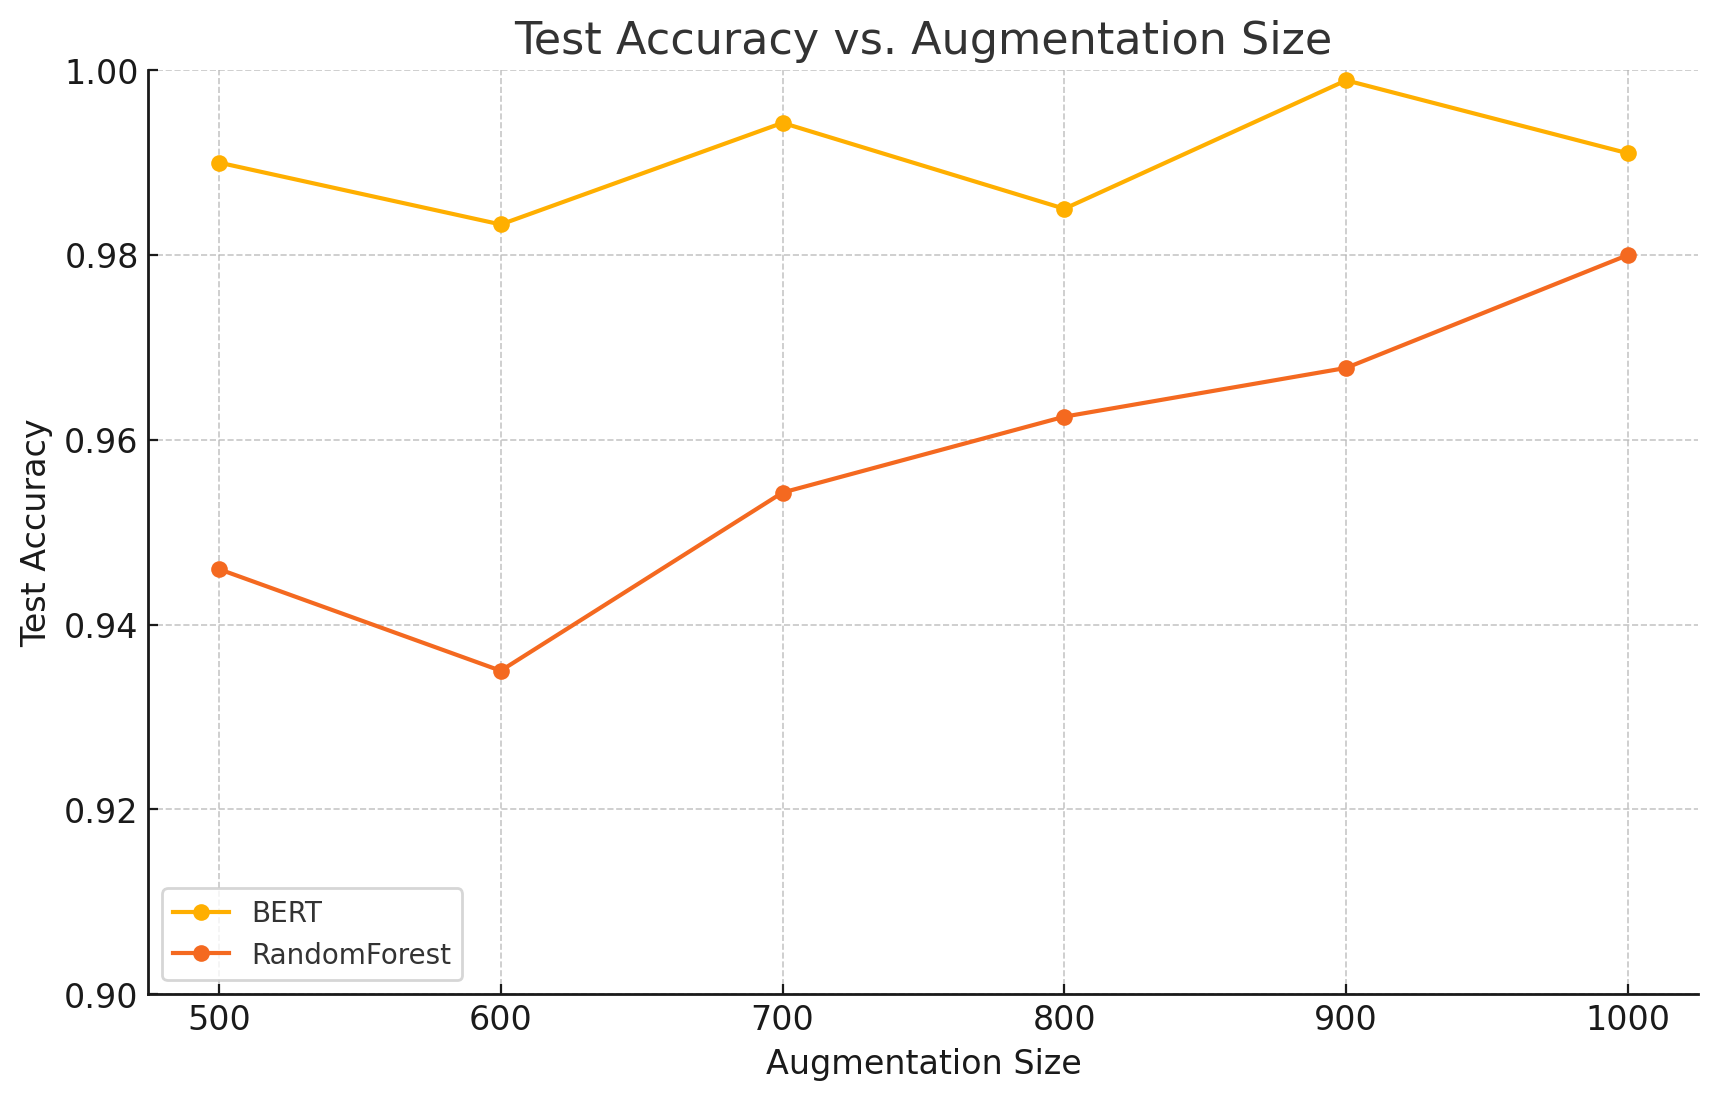
\includegraphics[width=12cm]{output (1).png}
%     \caption{%
%     The orange BERT curve starts above 0.99 and stays there, peaking at
%     900 augmented examples before tapering slightly. The red Random–Forest line begins almost five percentage points lower but rises steadily; by 1 000 examples it reaches 0.98, cutting the gap with BERT to barely 1.  This shows (i) deep models outperform classical ones when data are scarce, but (ii) inexpensive tree ensembles almost catch up once enough synthetic data are added—while remaining much lighter to train.}
% \end{figure}


% \begin{figure}[H]
%     \centering
%     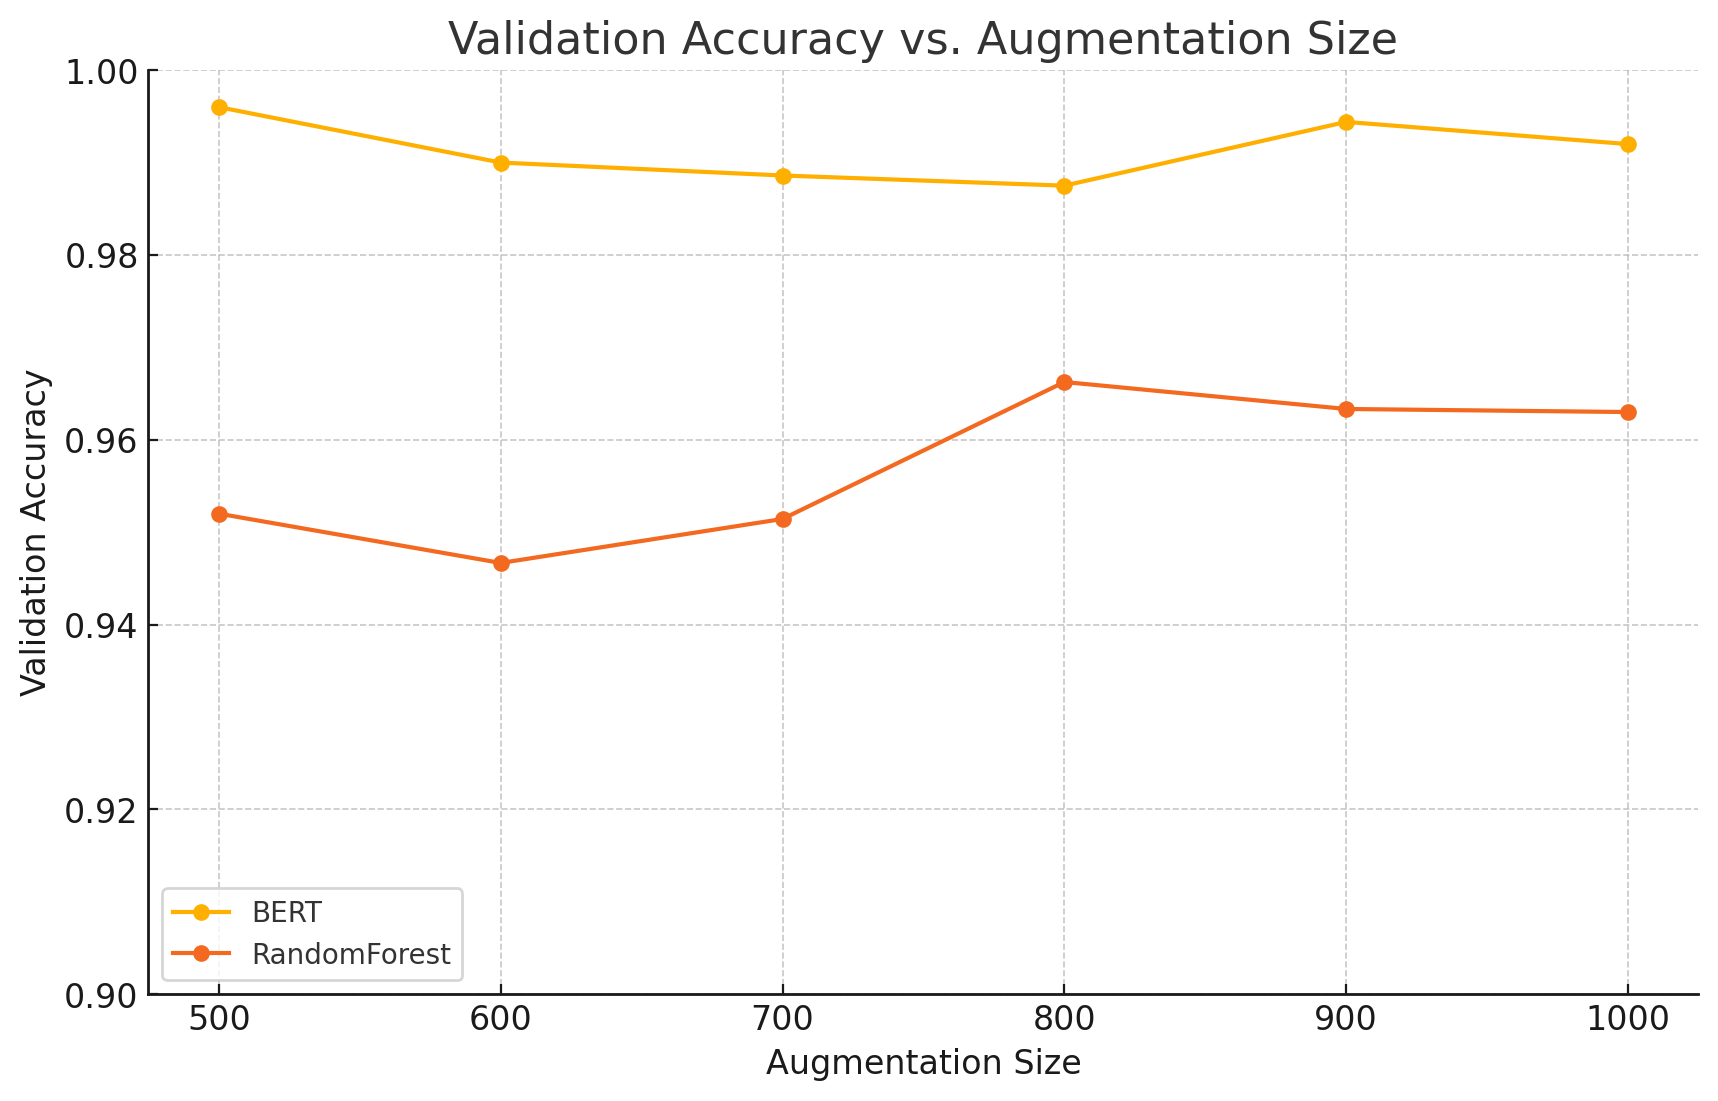
\includegraphics[width=12cm]{output (2).png}
%     \caption{%
%     Validation trends mirror the test curves but are less volatile. BERT is already at an accuracy of 0.995 with 500 extra samples and exhibits diminishing returns thereafter, hinting at a saturation point. Random Forest improves monotonically up to 800 samples, then flattens just below 0.965. This curve suggests that, beyond a certain size, additional augmentation contributes little generalisation gain—useful when deciding whether to keep generating synthetic data.
% }
% \end{figure}



% \begin{figure}[H]
%     \centering
%     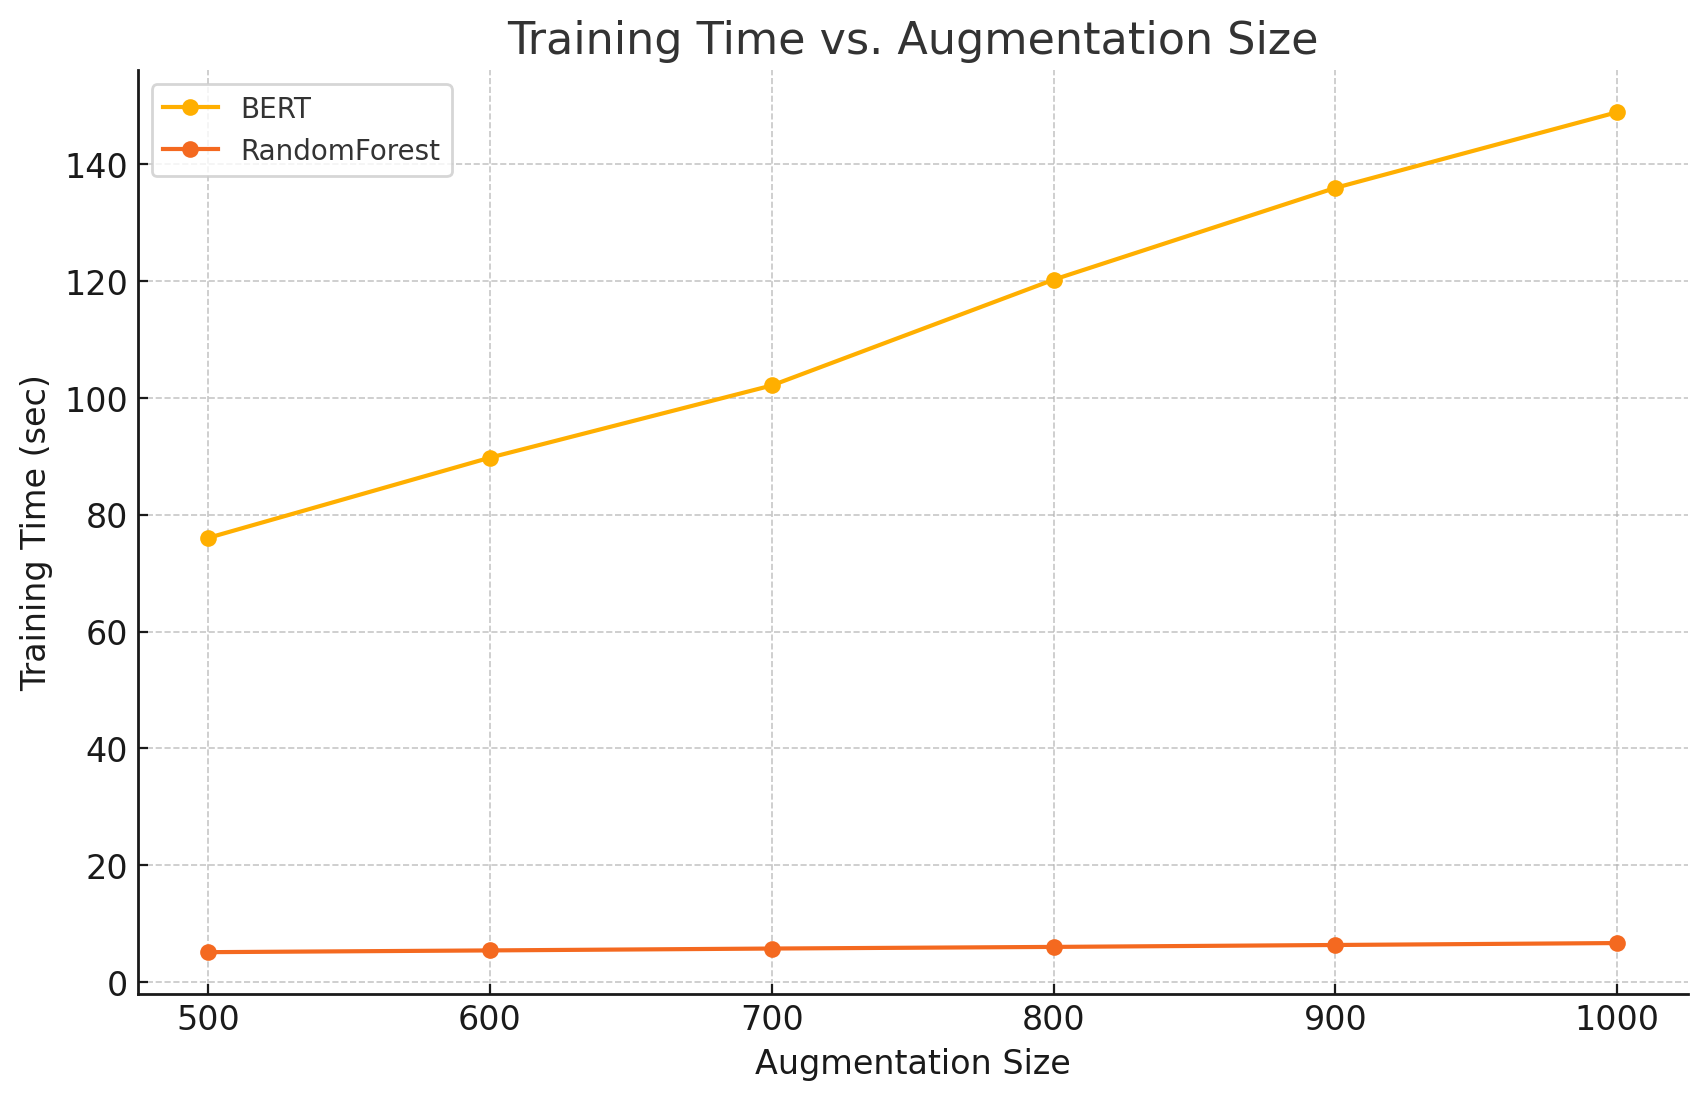
\includegraphics[width=12cm]{output (3).png}
%     \caption{%
%     Here the two lines diverge sharply. BERT’s training time climbs almost linearly from 75 s to 150 s as augmentation grows, reflecting the cost of fine-tuning a large Transformer. Random Forest, by contrast, inches up from 5 s to only 7 s, showing near-constant cost regardless of data volume. The takeaway: if wall-clock budget matters more than an extra percentage point of accuracy, the tree model offers a 20-to-1 speed advantage.}
% \end{figure}




% \begin{figure}[H]
%     \centering
%     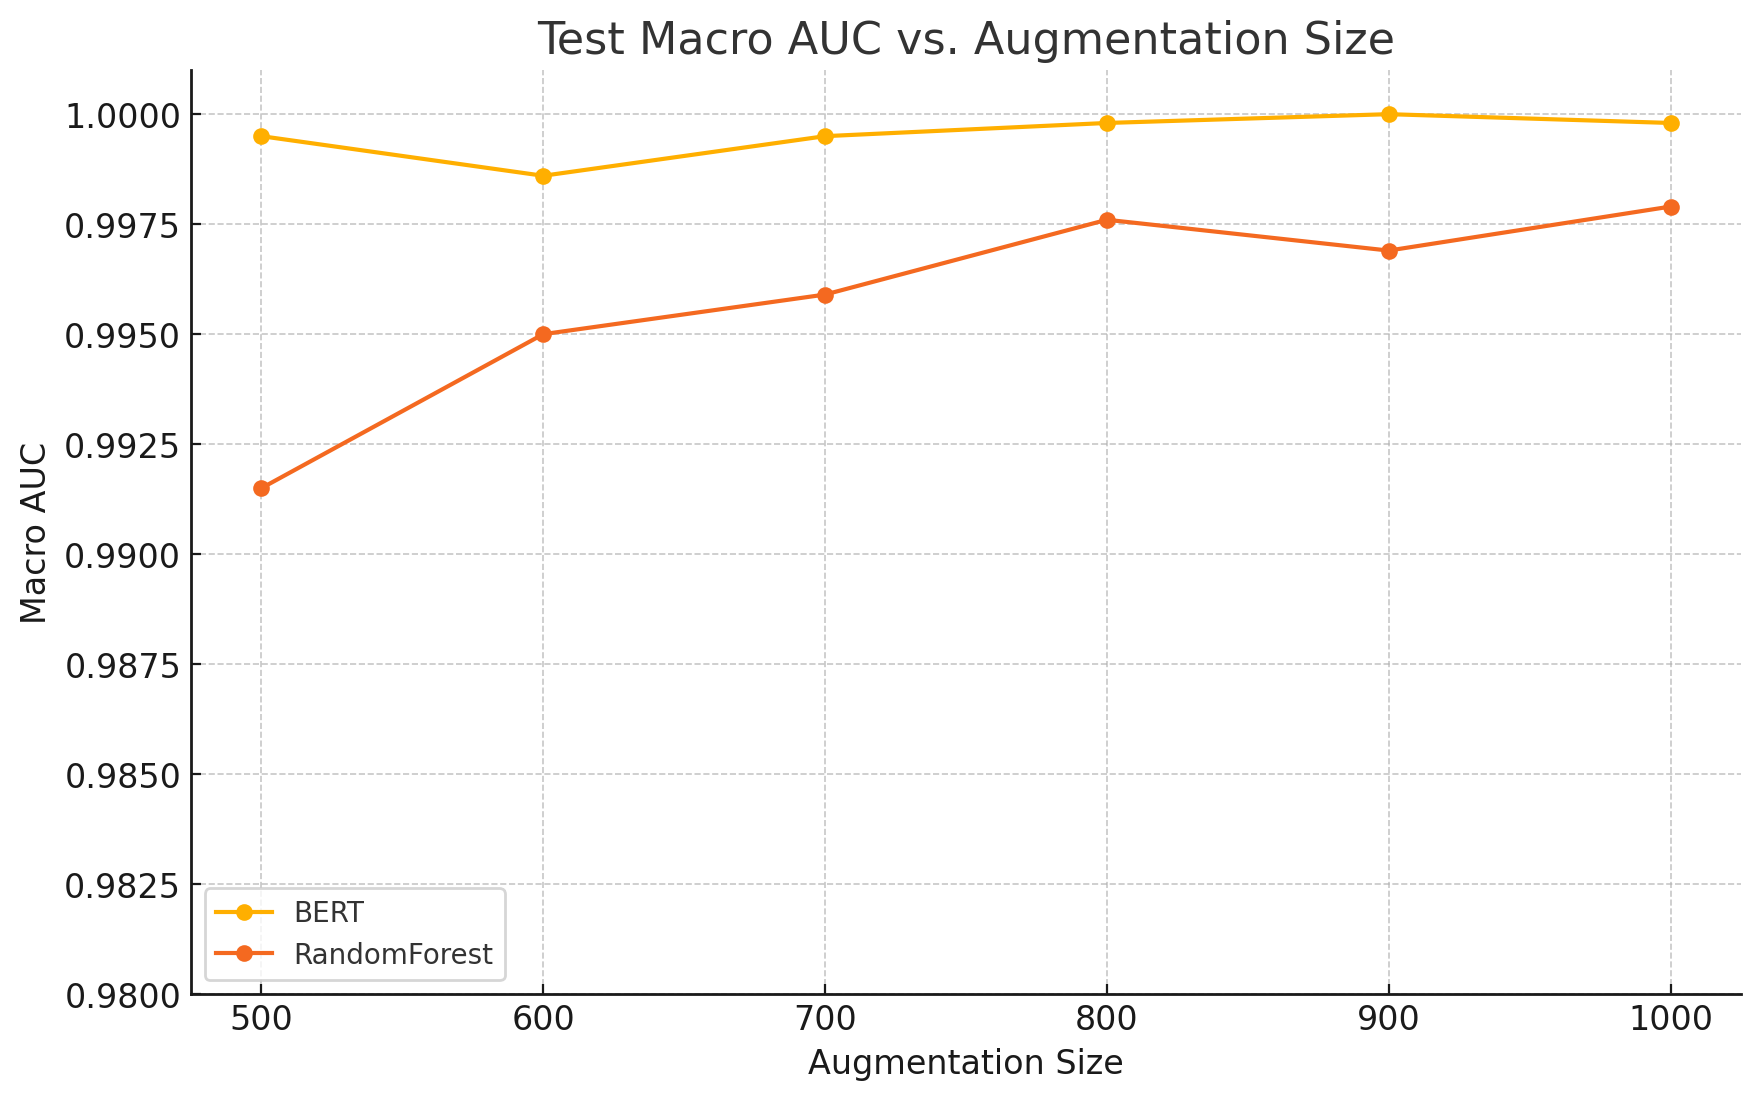
\includegraphics[width=12cm]{output (4).png}
%     \caption{%
%     Both models operate in the “top-right corner” of ROC space, yet BERT edges ahead. It is already at 0.9995 with 500 samples and reaches a perfect 1.000 at 900, after which gains saturate. Random Forest rises from 0.992 to 0.998 across the range, closing most of the initial gap. The curve highlights that ranking quality improves quickly with more data for RF, whereas BERT’s macro-AUC is effectively maxed out early on.}
% \end{figure}


% \begin{figure}[H]
%     \centering
%     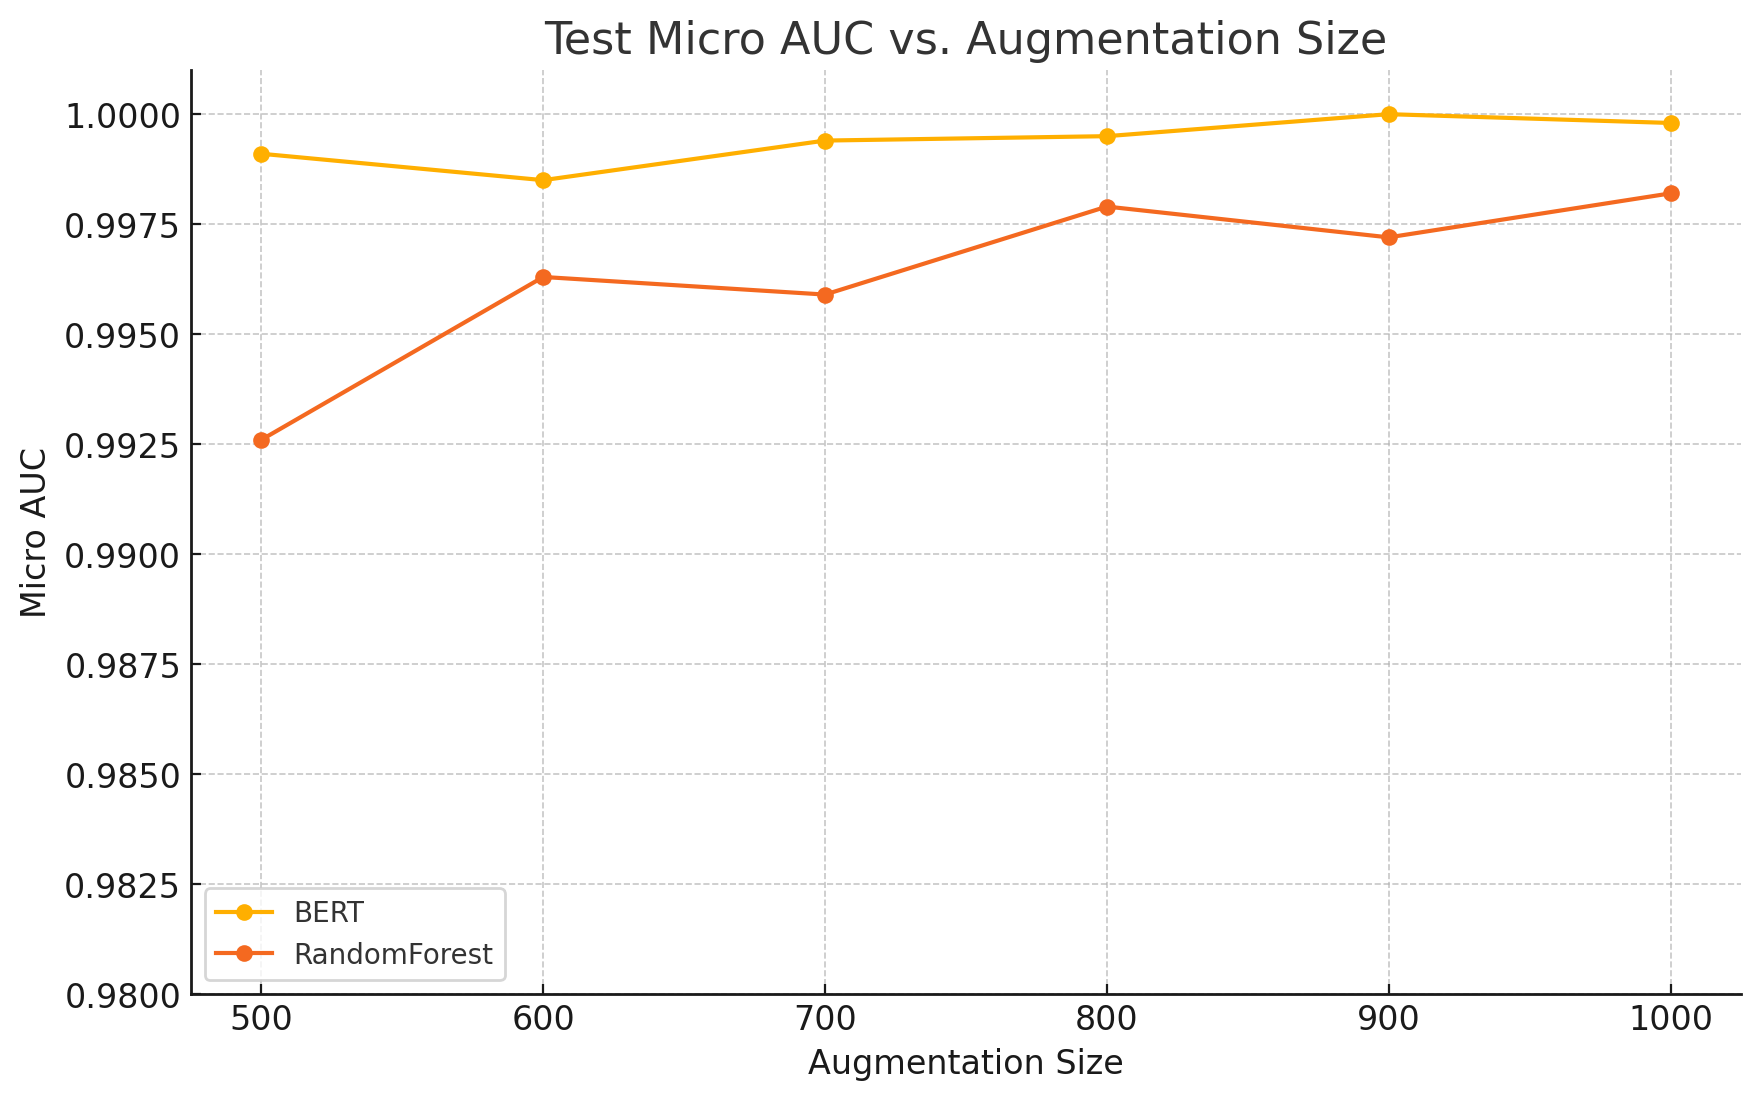
\includegraphics[width=12cm]{output (6).png}
%     \caption{%
%     The micro-AUC picture reinforces the macro view but is even tighter: BERT begins just under 0.999 and touches 1.000 at 900 augmentations; Random Forest progresses from about 0.992 to 0.998. Because micro-AUC weights classes by support, the convergence here indicates both models learn the majority classes extremely well. In operational terms, further optimisation should focus on class-specific precision-recall trade-offs rather than overall ranking capability, which is already near-perfect.}
% \end{figure}


Deep models such as BERT outperform classical models when data are scarce, achieving over 0.99 test accuracy with limited augmentation. In contrast, Random Forest starts with a noticeable gap but steadily improves as more synthetic data are added, ultimately reaching 0.98 and closing most of the performance difference. This highlights that although BERT offers a clear early advantage, lightweight models can become competitive with sufficient augmentation, providing a more computationally efficient alternative (Figure~\ref{fig:test_accuracy}).


\begin{figure}[H]
    \centering
    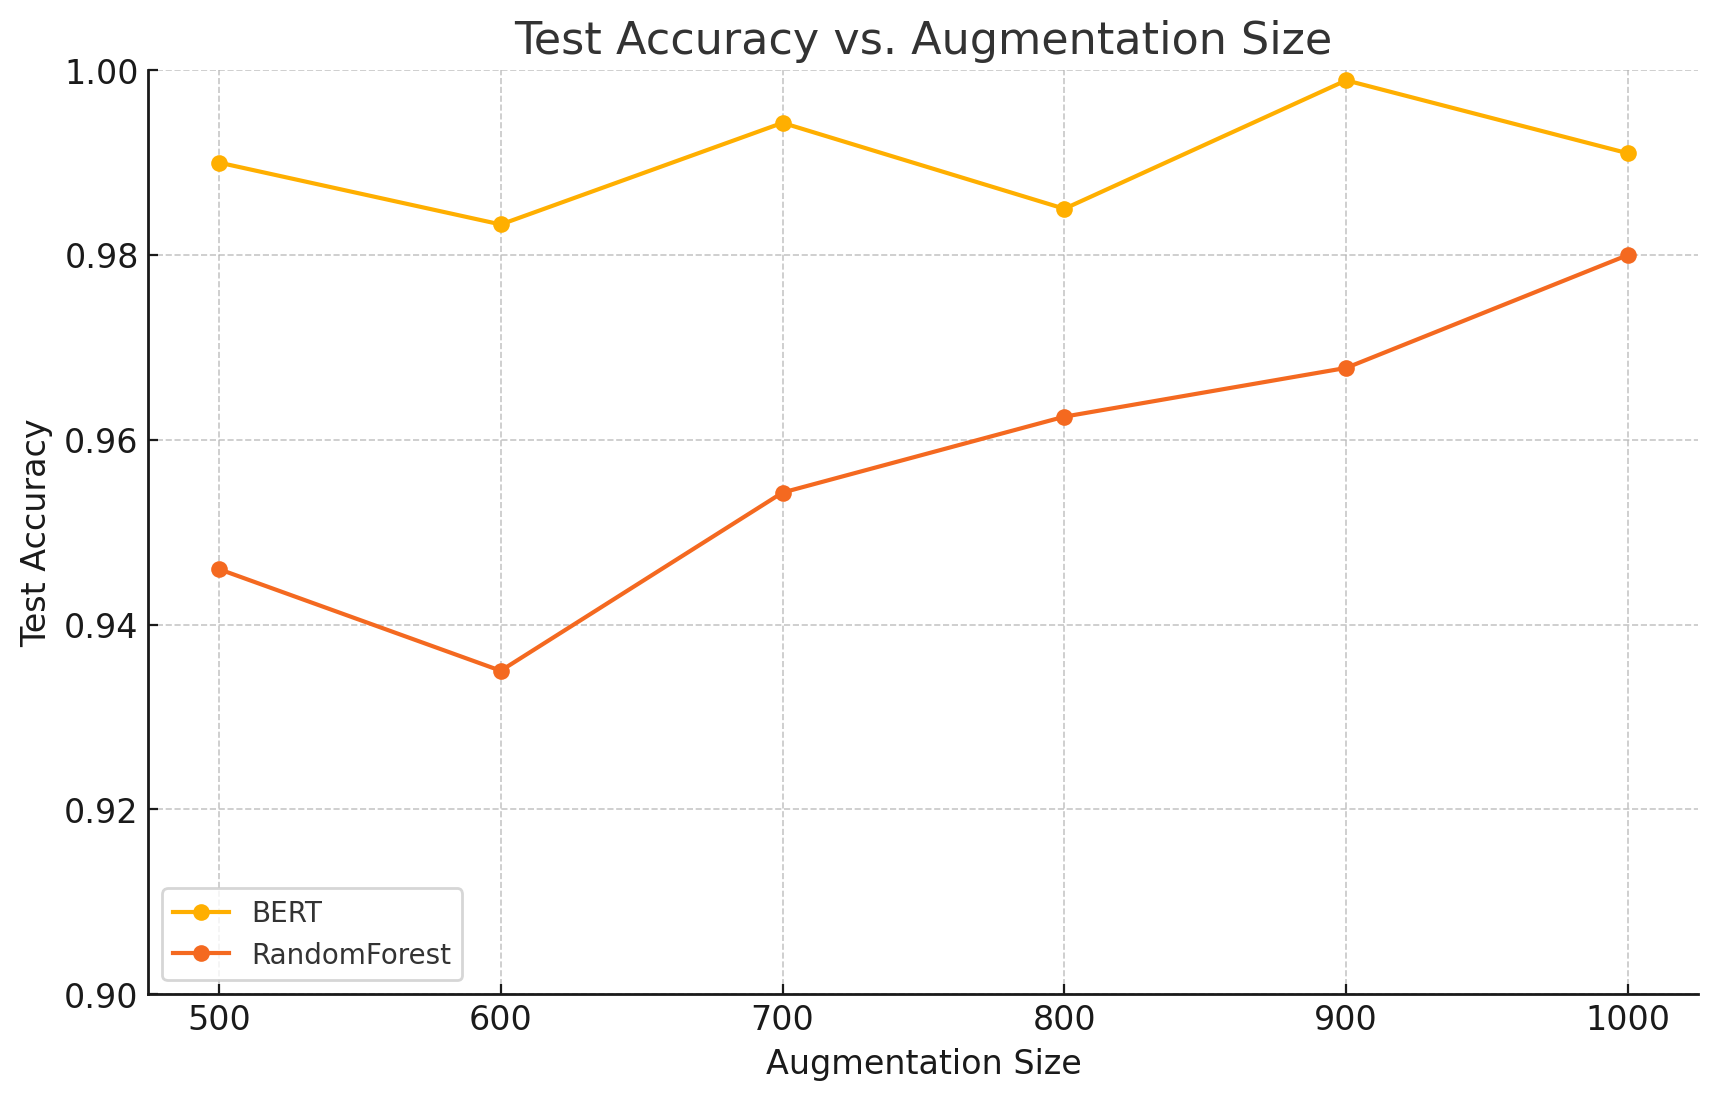
\includegraphics[width=10cm]{output (1).png}
    \caption{Test accuracy trends for BERT and Random Forest as a function of augmented sample size. BERT consistently outperforms Random Forest when data are scarce, but the gap narrows significantly with larger augmentation.}
    \label{fig:test_accuracy}
\end{figure}

BERT achieves a validation accuracy of 0.995 with only 500 training samples, after which additional data offer diminishing returns, suggesting a saturation point. Random Forest continues to improve up to around 800 samples before flattening just below 0.965. These trends indicate that beyond a certain augmentation size, further synthetic data provide minimal generalization benefits (Figure~\ref{fig:validation_accuracy}).


\begin{figure}[H]
    \centering
    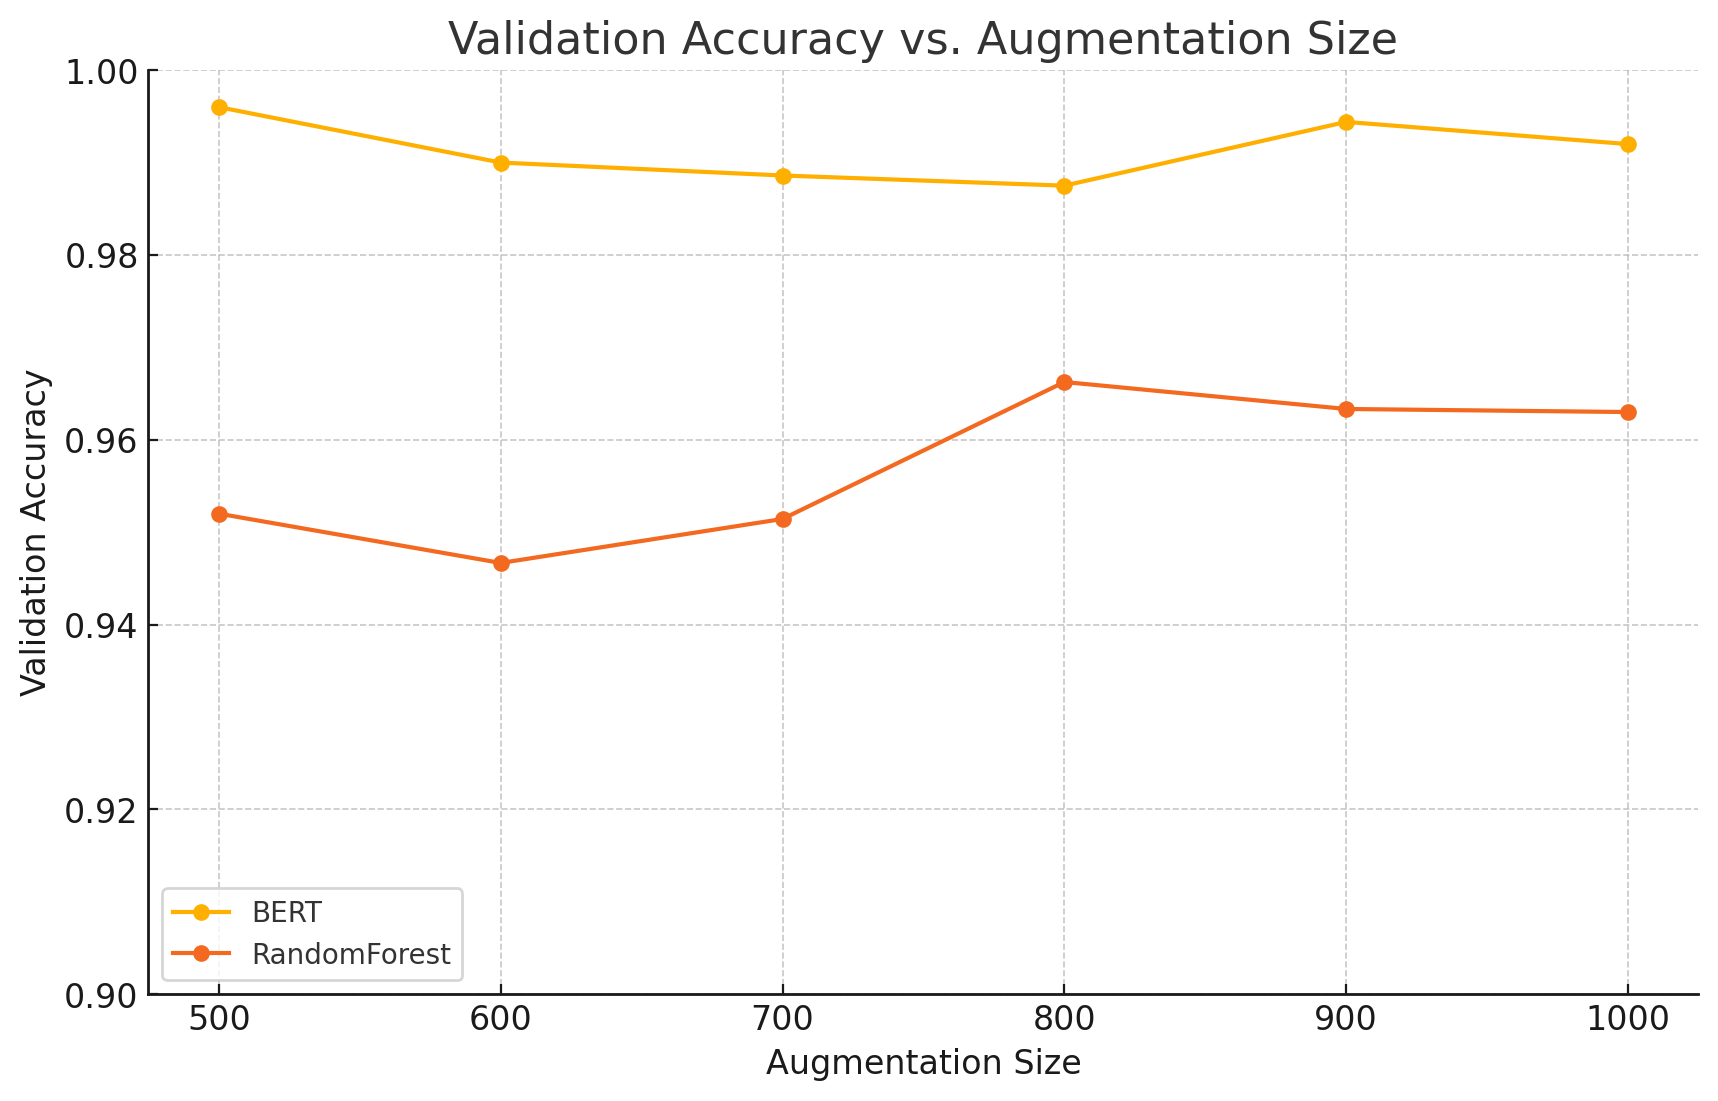
\includegraphics[width=10cm]{output (2).png}
    \caption{Validation accuracy for BERT and Random Forest under increasing augmentation. BERT saturates earlier, whereas Random Forest sees gradual gains before reaching the saturation.}
    \label{fig:validation_accuracy}
\end{figure}

In terms of computational cost, BERT’s training time increases nearly linearly from 75 to 150 seconds as augmentation increases, reflecting the growing cost of fine-tuning a large Transformer model. In contrast, Random Forest maintains a near-constant runtime, rising only from 5 to 7 seconds. When computational efficiency is a priority, Random Forest offers a roughly 20-to-1 speed advantage over BERT (Figure~\ref{fig:training_time}). This demonstrates the potential application of random forest-based model in the instant real-world emotional classification tasks. 


\begin{figure}[H]
    \centering
    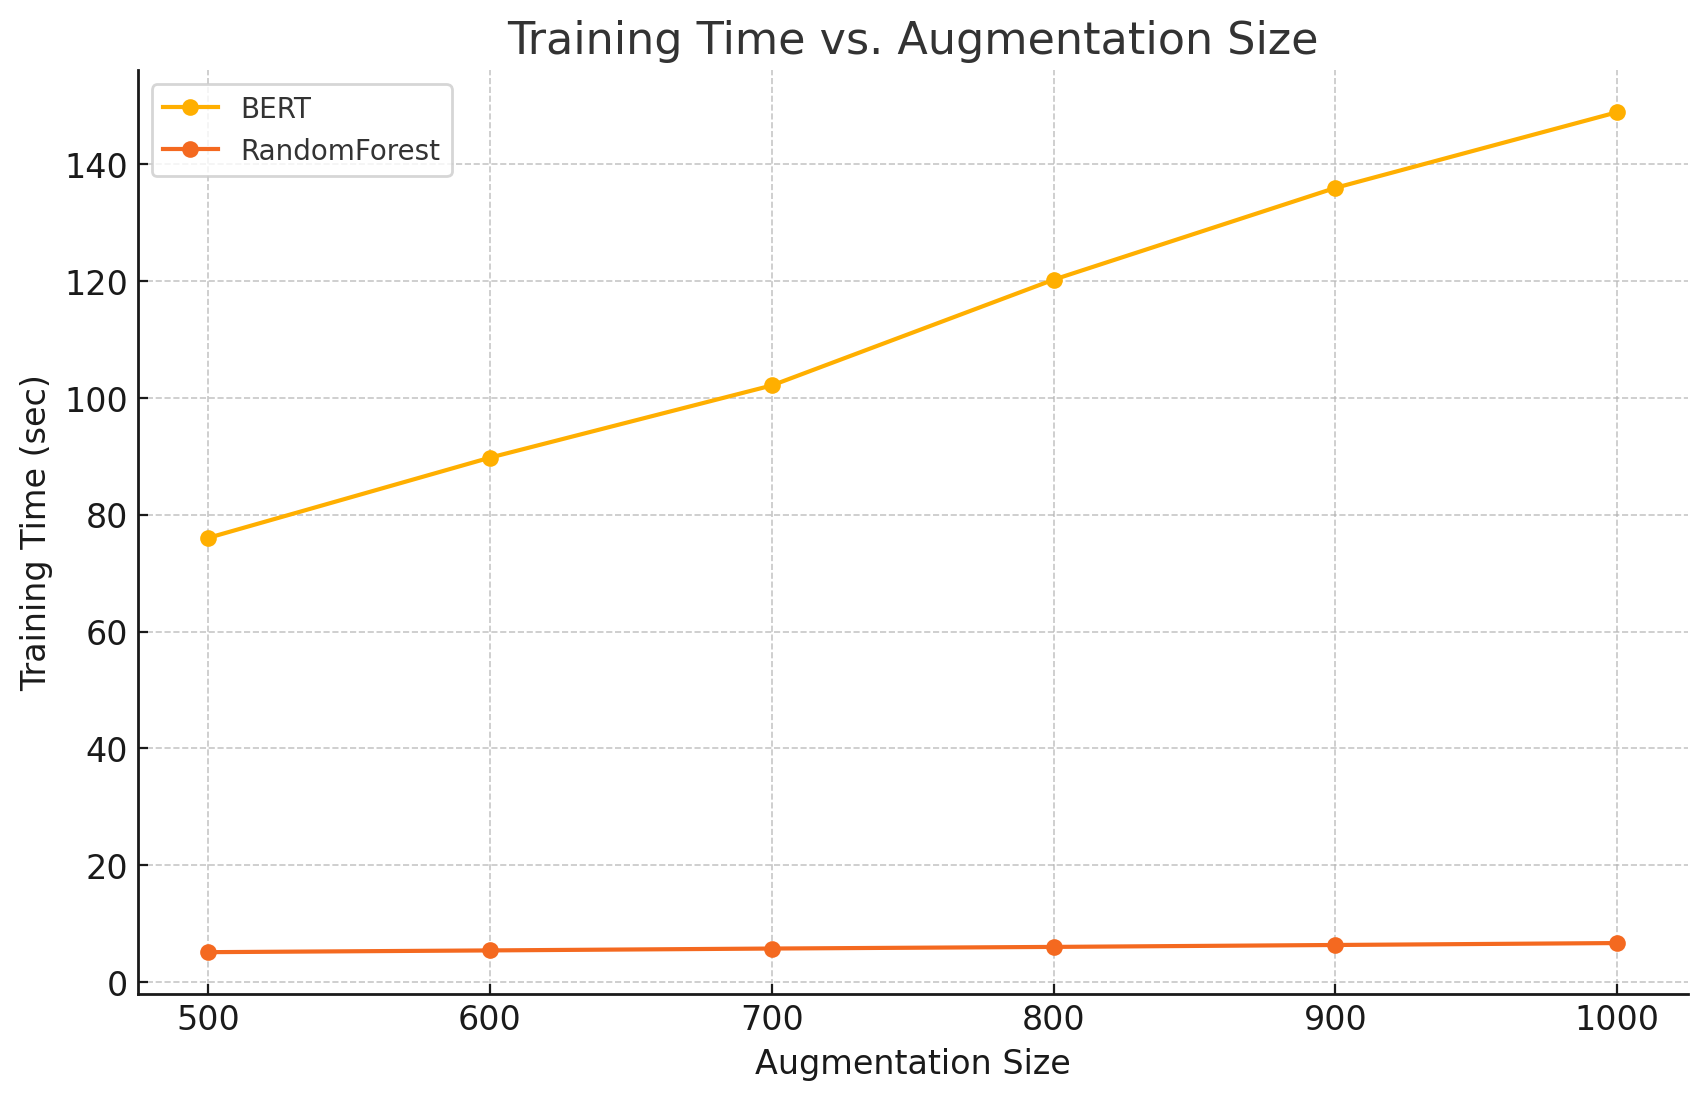
\includegraphics[width=10cm]{output (3).png}
    \caption{Training time as a function of augmented data volume. BERT exhibits a near-linear increase, whereas Random Forest remains almost constant.}
    \label{fig:training_time}
\end{figure}

BERT achieves near-perfect macro-AUC with only 500 augmented samples and saturates at 1.000 by 900. Random Forest starts lower but steadily improves from 0.992 to 0.998 as more data are added. These results suggest that BERT reaches optimal ranking performance early, while Random Forest continues to gain from additional augmentation (Figure~\ref{fig:macro_auc}).


\begin{figure}[H]
    \centering
    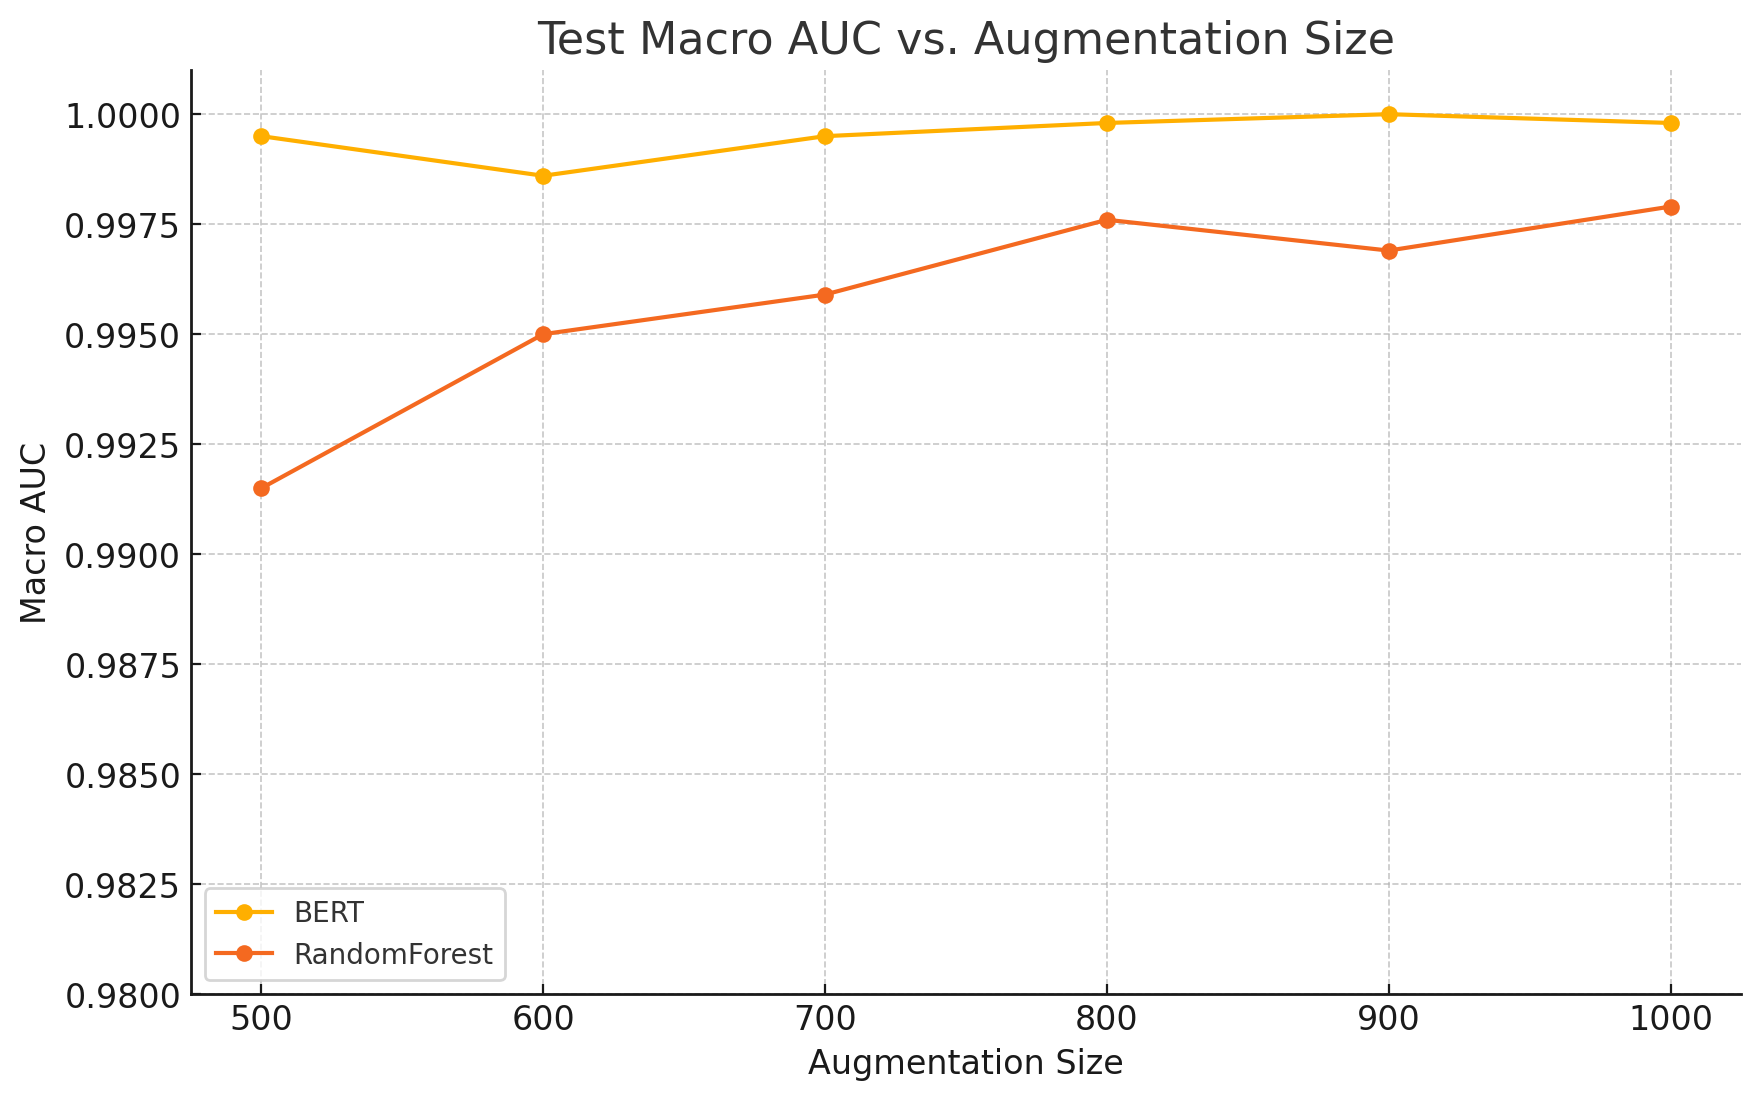
\includegraphics[width=10cm]{output (4).png}
    \caption{Macro-AUC performance for BERT and Random Forest with increasing augmentation. BERT saturates earlier, while Random Forest closes much of the initial gap.}
    \label{fig:macro_auc}
\end{figure}

BERT reaches nearly 1.000 micro-AUC by 900 augmentations, while Random Forest improves from approximately 0.992 to 0.998. Since micro-AUC accounts for class support, this tight convergence indicates that both models perform exceptionally well on majority classes. Further optimization should therefore focus on class-specific metrics such as precision and recall rather than overall ranking performance (Figure~\ref{fig:micro_auc}).


\begin{figure}[H]
    \centering
    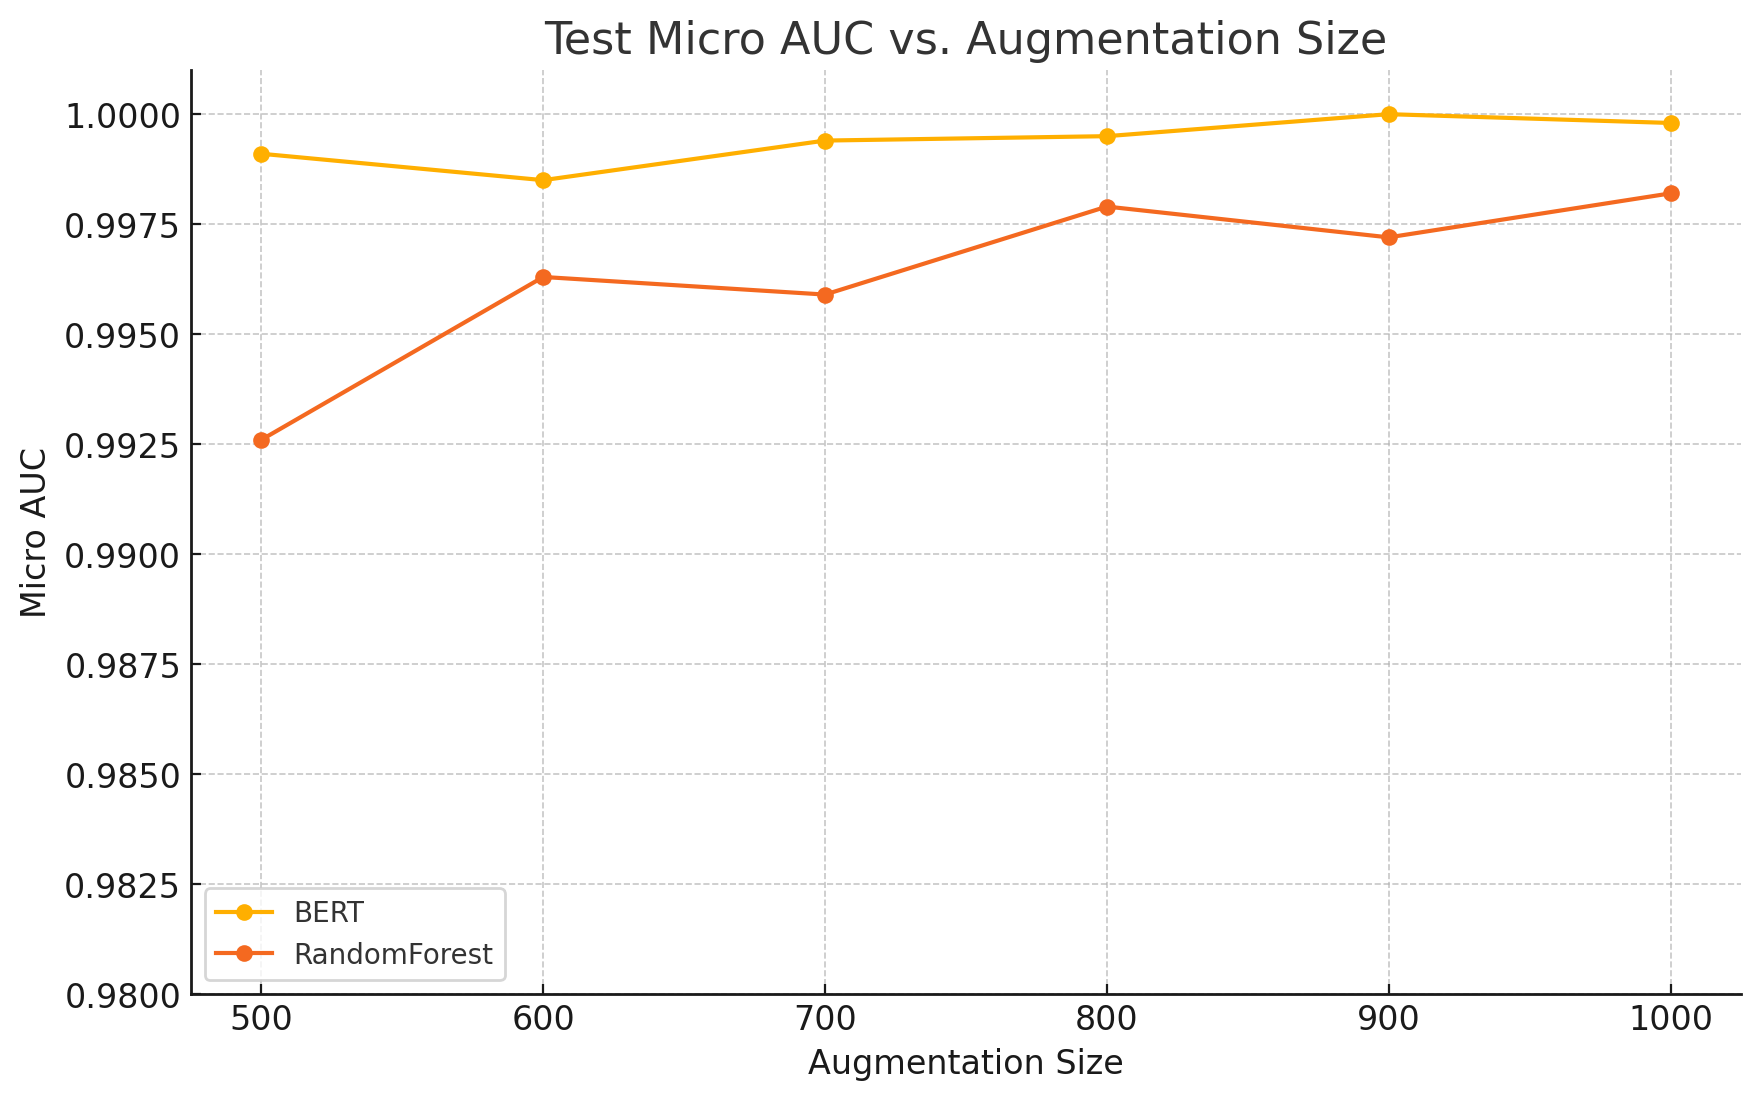
\includegraphics[width=10cm]{output (6).png}
    \caption{Micro-AUC performance for BERT and Random Forest. Both models achieve near-perfect scores, with BERT saturating faster.}
    \label{fig:micro_auc}
\end{figure}


\section{Discussion and Conclusion}
This project addressed the challenge of classifying emotions (joy, sadness, anger, love, fear, surprise) in Twitter comments using a dataset expanded via LLM-based data augmentation. This augmentation proved crucial for improving model performance, particularly given the initial limitations of labeled data. We compared a deep learning model (BERT) with a classical machine learning model (Random Forest, RF). 

It is worth noting that our initial process did not involve human verification to ensure data quality. As a result, biases introduced during data collection, such as user-labeled errors or advertisements containing multiple conflicting labels, were mistakenly included in the training set. This contamination degraded the quality of both the original and augmented datasets, significantly increasing the difficulty for predictive models. Under these conditions, Random Forest achieved only around 80\% accuracy, and surprisingly, BERT performed even worse at around 75\%. We hypothesize that this occurred because BERT more effectively learned incorrect sentence-label mappings, leading to inferior performance compared to traditional machine learning methods.

To address this issue, we introduced a human verification step. Additionally, during data augmentation, we chose not to strictly forbid large language models from generating sentences with explicit emotional expressions. This decision was motivated by two considerations: (1) direct emotional expressions are common in everyday language and including them can improve model adaptability, and (2) overly relying on subtle emotional expressions increased the chance of label overlap and confusion, such as confusion between \textit{joy} and \textit{love}, or \textit{fear} and \textit{anger}. In real-world settings, even human could not precisely distinguish these subtle emotional boundaries, frequently categorizing a sentence as representing multiple emotions simultaneously. As a result, forcing the model to predict only a single emotion in such cases would be unreasonable.

After implementing these corrections, the model accuracy improved to the results reported in this study. It also showed that data augmentation significantly boosted the performance of both models, allowing them to achieve high accuracy ($>$ 0.98) and AUC scores ($>$ 0.998). BERT demonstrated slightly higher accuracy and AUC, especially with less augmentation, confirming the power of deep learning approaches. However, this came at a considerably higher computational cost, with training time increasing linearly with data size. Conversely, Random Forest's performance improved dramatically with augmented data, nearly matching BERT's accuracy while remaining significantly faster and more computationally efficient. We observed diminishing returns from augmentation beyond a certain point, suggesting a saturation effect. 

In conclusion, this study demonstrates that LLM-based data augmentation is an effective strategy to overcome data scarcity in text classification tasks such as emotion detection in tweets. With sufficient augmentation, both complex models like BERT and simpler models like Random Forest can achieve strong performance. While BERT achieves peak accuracy, Random Forest offers a computationally efficient alternative when project constraints favor faster, lighter models. These findings highlight a practical trade-off between model complexity and resource usage, and support the application of such methods to real-world sentiment and emotion analysis systems.
 

\section{Code Availability}
The code developed for this project is publicly available on GitHub at the following repository:
\url{https://github.com/xiaohuang-6/NLP_emotional_classification/tree/main}


\section{Contributions}
\begin{itemize}
    \item \textbf{Chengkun Yang, Yitao Shi:} Data collection and preprocessing; implemented initial exploratory data analysis scripts.
    \item \textbf{Yue(Joey) Yu:} Led model development and training for both classical and deep learning approaches; responsible for hyperparameter tuning and evaluation.
    \item \textbf{Chengkun Yang, Xiao Huang and Teng-yu (Echo) Hsiao:} Written this report; assisted in data cleaning and model validation; prepared presentation slides.
\end{itemize}

\newpage

\bibliographystyle{alpha}
\bibliography{sample}

\end{document}